% Draslovka — introduction deck (3 slides, Beamer, 16:9)
%   1) primer: what retrosynthesis IS, on one of their own molecules
%   2) the toolbox: each tool is partial; our objective is the ladder + active learning
%   3) where these methods pay off -- GENERAL, deliberately not company-targeted
% Build:  pdflatex intro-deck.tex   (single run; no bibliography, no external assets)
%
% AUDIENCE = Draslovka managers. Bar is competence, not novelty.
%
% WHAT MUST NOT GO BACK IN (owner instruction, 2026-07-29):
%   * no count of our own failures ("three attempts failed", "every run exhausted its budget");
%   * no calibration / "knows what it doesn't know" capability claim.
% Escalation is justified by TOOLS DISAGREEING -- an observable -- not by a model-internal
% confidence signal we do not have. Active learning is presented as the research OBJECTIVE,
% and extends to EXPERIMENTAL active learning (which experiment to run next).
% See ../STATUS.md, "Claims that must now come OUT of the pitch".
%
% Colour never carries meaning alone: every status is a WORD, tinted.

\documentclass[aspectratio=169,11pt]{beamer}

\usepackage[T1]{fontenc}
\usepackage[utf8]{inputenc}
\usepackage{lmodern}
\usepackage{booktabs}
\usepackage{tabularx}
\usepackage[version=4]{mhchem}
\usepackage{tikz}
\usetikzlibrary{arrows.meta, positioning, fit, backgrounds}

% ---- intermediate type scale -------------------------------------------------
% Beamer only offers 10/11/12pt base sizes. This deck wants to sit BETWEEN its
% 10pt and 11pt versions, so the two sizes actually used for slide text are set
% explicitly. Body was 9pt (10pt base) then 10pt (11pt base) -> 9.5pt here;
% annotations were 7pt then 8pt -> 7.6pt; frame title was 12pt then 14.4pt -> 13.2pt.
% Change these three numbers to rescale the whole deck.
\makeatletter
\renewcommand{\small}{\@setfontsize\small{9.5}{11.6}}
\renewcommand{\scriptsize}{\@setfontsize\scriptsize{7.6}{9.2}}
\makeatother
\newcommand{\ftsize}{\fontsize{13.2}{15.8}\selectfont}

\usetheme{default}
\usecolortheme{default}
\setbeamertemplate{navigation symbols}{}
\setbeamerfont{frametitle}{size=\ftsize, series=\bfseries}
\setbeamerfont{framesubtitle}{size=\small, series=\mdseries}
\makeatletter
\setbeamertemplate{frametitle}{%
  \vskip3pt\usebeamerfont{frametitle}\usebeamercolor[fg]{frametitle}\insertframetitle\par
  \ifx\insertframesubtitle\@empty\else
    \vskip2pt{\usebeamerfont{framesubtitle}\usebeamercolor[fg]{framesubtitle}\insertframesubtitle\par}
  \fi\vskip3pt}
\makeatother

\definecolor{accent}{HTML}{2A78D6}
\definecolor{ink}{HTML}{0B0B0B}
\definecolor{ink2}{HTML}{52514E}
\definecolor{ink3}{HTML}{7A7975}
\definecolor{rule}{HTML}{E3E2DD}
\definecolor{plane}{HTML}{F4F4F1}
\definecolor{good}{HTML}{006300}
\definecolor{bad}{HTML}{D03B3B}

\setbeamercolor{normal text}{fg=ink}
\setbeamercolor{frametitle}{fg=ink, bg=}
\setbeamercolor{framesubtitle}{fg=ink2}
\usebeamercolor[fg]{normal text}

\newcommand{\mature}[1]{{\color{good}\bfseries #1}}
\newcommand{\early}[1]{{\color{accent}\bfseries #1}}
\newcommand{\caveat}[1]{{\color{bad}\bfseries #1}}
\newcommand{\lead}[1]{{\color{accent}\bfseries #1}}

\begin{document}
\setlength{\parskip}{0pt}

% ============================================================ SLIDE 1 (primer)
% Worked example is Draslovka's OWN value chain read backwards:
% hydantoin <- acetone cyanohydrin <- HCN. Every step is real industrial chemistry,
% and our own audit independently confirmed the cyanohydrin step sound
% (see ../experiments/RESULTS.md). Do not swap in a pharma molecule -- the point
% is that the method reproduces chemistry they already run.
{\setbeamercolor{background canvas}{bg=white}
\begin{frame}[t]{What is retrosynthesis?}{Planning a synthesis \emph{backwards} --- from the molecule you want, to things you can buy}

\vspace{0pt}
\begin{columns}[t, onlytextwidth]
\begin{column}{0.56\textwidth}
\begin{center}
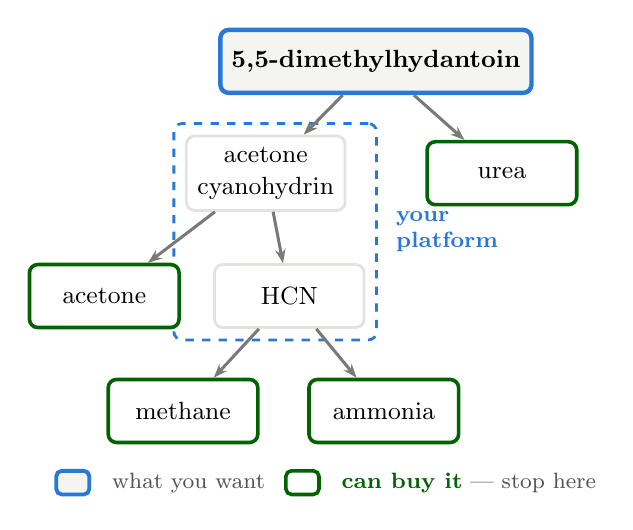
\begin{tikzpicture}[
  font=\small,
  mol/.style={draw=rule, line width=1pt, fill=white, rounded corners=3pt,
              align=center, inner sep=4pt, minimum height=8mm, minimum width=19mm},
  tgt/.style={mol, draw=accent, line width=1.6pt, fill=plane, font=\small\bfseries},
  buy/.style={mol, draw=good, line width=1.3pt},
  ar/.style={-{Stealth[length=5pt]}, draw=ink3, line width=1.1pt}
]
  \node[tgt] (dmh) at (0,0)          {5,5-dimethylhydantoin};
  \node[mol] (ach) at (-1.4,-1.42)   {acetone\\cyanohydrin};
  \node[buy] (urea) at (1.6,-1.42)   {urea};
  \node[buy] (acet) at (-3.45,-2.98)  {acetone};
  \node[mol] (hcn)  at (-1.1,-2.98)  {\ce{HCN}};
  \node[buy] (met)  at (-2.45,-4.44)  {methane};
  \node[buy] (nh3)  at (0.1,-4.44)  {ammonia};

  \begin{scope}[on background layer]
    \node[draw=accent, dashed, line width=1pt, rounded corners=3pt,
          inner sep=4pt, fit=(ach)(hcn)] (spine) {};
  \end{scope}
  \node[anchor=west, font=\scriptsize\bfseries, color=accent, align=left]
        at ([xshift=3pt]spine.east) {your\\platform};

  \draw[ar] (dmh) -- (ach);   \draw[ar] (dmh) -- (urea);
  \draw[ar] (ach) -- (acet);  \draw[ar] (ach) -- (hcn);
  \draw[ar] (hcn) -- (met);   \draw[ar] (hcn) -- (nh3);

  \node[draw=accent, line width=1.4pt, fill=plane, rounded corners=2pt,
        minimum width=4.2mm, minimum height=3mm, inner sep=0pt] (k1) at (-3.85,-5.35) {};
  \node[anchor=west, font=\scriptsize, color=ink2] (k1t) at ([xshift=4pt]k1.east) {what you want};
  \node[draw=good, line width=1.3pt, fill=white, rounded corners=2pt,
        minimum width=4.2mm, minimum height=3mm, inner sep=0pt] (k2) at ([xshift=10pt]k1t.east) {};
  \node[anchor=west, font=\scriptsize, color=ink2] at ([xshift=4pt]k2.east)
        {\textcolor{good}{\bfseries can buy it} --- stop here};
\end{tikzpicture}
\end{center}
\end{column}

\begin{column}{0.42\textwidth}
\vspace{8pt}
{\small
{\color{accent}\bfseries 1.}\; Each arrow is one reaction. Read \textbf{backwards}: \emph{the boxes
below make the box above}.\par\vskip8pt
{\color{accent}\bfseries 2.}\; Stop when you reach something you can \textbf{buy}.\par\vskip8pt
{\color{accent}\bfseries 3.}\; The spine is \textbf{your own value chain} --- \ce{HCN} to cyanohydrin
to hydantoin.\par\vskip11pt
\colorbox{plane}{\parbox{\dimexpr\linewidth-10pt\relax}{\small
{\color{bad}\bfseries The catch.} Enumerating these trees is easy. Knowing which arrows \emph{work in
a reactor} is not --- and that is the rest of this talk.}}}
\end{column}
\end{columns}

\end{frame}}

% ======================================================= SLIDE 2 (the toolbox)
\begin{frame}[t]{The tools that exist --- and why none of them is enough}{Each one is strong exactly where the others are blind. The opportunity is in \emph{combining} them.}

\vspace{2pt}
\begin{center}
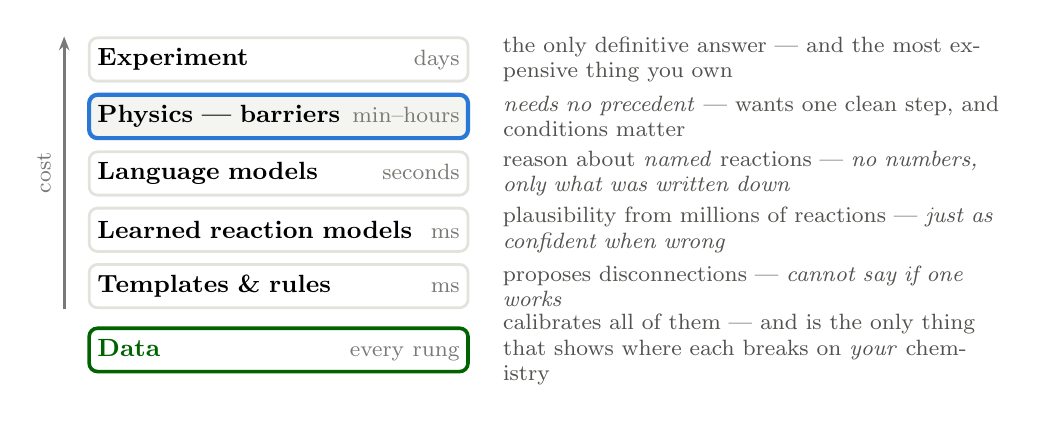
\begin{tikzpicture}[
  font=\small,
  rung/.style={draw=rule, line width=1pt, fill=white, rounded corners=3pt,
               text width=46mm, align=left, inner sep=3pt, minimum height=5.5mm},
  phys/.style={rung, draw=accent, line width=1.5pt, fill=plane},
  lim/.style={anchor=west, font=\scriptsize, color=ink2, align=left, text width=63mm},
  cost/.style={-{Stealth[length=5pt]}, draw=ink3, line width=1.2pt}
]
  \node[rung] (r1) at (0,0) {\textbf{Templates \& rules}\hfill{\scriptsize\color{ink3}ms}};
  \node[rung, above=1.3mm of r1] (r2) {\textbf{Learned reaction models}\hfill{\scriptsize\color{ink3}ms}};
  \node[rung, above=1.3mm of r2] (r3) {\textbf{Language models}\hfill{\scriptsize\color{ink3}seconds}};
  \node[phys, above=1.3mm of r3] (r4) {\textbf{Physics --- barriers}\hfill{\scriptsize\color{ink3}min--hours}};
  \node[rung, above=1.3mm of r4] (r5) {\textbf{Experiment}\hfill{\scriptsize\color{ink3}days}};

  \node[lim] at ([xshift=3mm]r1.east) {proposes disconnections --- \emph{cannot say if one works}};
  \node[lim] at ([xshift=3mm]r2.east) {plausibility from millions of reactions --- \emph{just as confident when wrong}};
  \node[lim] at ([xshift=3mm]r3.east) {reason about \emph{named} reactions --- \emph{no numbers, only what was written down}};
  \node[lim] at ([xshift=3mm]r4.east) {\emph{needs no precedent} --- wants one clean step, and conditions matter};
  \node[lim] at ([xshift=3mm]r5.east) {the only definitive answer --- and the most expensive thing you own};

  \draw[cost] ([xshift=-3mm]r1.south west) -- ([xshift=-3mm]r5.north west)
        node[midway, rotate=90, anchor=south, font=\scriptsize, color=ink3, yshift=1pt] {cost};

  \node[draw=good, line width=1.3pt, fill=white, rounded corners=3pt,
        text width=46mm, align=left, inner sep=3pt, minimum height=5.5mm,
        below=2.2mm of r1] (dat) {\textbf{\textcolor{good}{Data}}\hfill{\scriptsize\color{ink3}every rung}};
  \node[lim] at ([xshift=3mm]dat.east) {calibrates all of them --- and is the only thing that shows where each breaks on \emph{your} chemistry};
\end{tikzpicture}
\end{center}

\vspace{4pt}
\colorbox{plane}{\parbox{\dimexpr\textwidth-10pt\relax}{\small
\lead{Our objective is the ladder.}\; Send each question to the \textbf{cheapest tool that can answer
it}; climb a rung only where the tools \textbf{disagree} --- an observable, with no model grading its
own homework.
\par\vskip3pt
\early{Active learning is the research.}\; \emph{What} to escalate is the open question we work on ---
for computation, and then for \textbf{which experiment to run next}.}}

\end{frame}

% ==================================================================== SLIDE 3
\begin{frame}[t]{Where these methods pay off}{Four recurring needs in industrial process chemistry --- ranked by what is ready today}

\vspace{2pt}
\renewcommand{\arraystretch}{1.05}
\begin{tabularx}{\textwidth}{@{}>{\raggedright\small\arraybackslash}p{0.215\textwidth}
                               >{\small}X
                               >{\raggedright\small\arraybackslash}p{0.155\textwidth}@{}}
\toprule
{\scriptsize\bfseries\color{ink3} INDUSTRIAL NEED} &
{\scriptsize\bfseries\color{ink3} WHAT THE METHODS OFFER} &
{\scriptsize\bfseries\color{ink3} MATURITY} \\
\midrule

\textbf{Greener or cheaper route} &
Route search \emph{under a constraint} --- avoid a reagent, cut cost or hazard. &
\lead{High impact} \\

\textbf{Lab-to-industrial routes} &
Feasibility-ranked routes to a chosen target, with an explicit ``cannot judge'' bucket. &
\mature{Most mature} \\

\textbf{Viability in real conditions} &
First-principles \emph{barriers}: kinetics, not thermodynamics. &
\early{Differentiating} \\

\textbf{Feedstock valorisation} &
Proposing higher-value targets reachable from a cheap feedstock. &
\caveat{Roadmap only} \\
\bottomrule
\end{tabularx}

\vspace{6pt}
\colorbox{plane}{\parbox{\dimexpr\textwidth-10pt\relax}{\small
\caveat{The caveat we would rather raise ourselves.}\; Public reaction models --- ours included --- learn
from patent literature that is heavily organic and pharmaceutical, so \textbf{specialty and process
chemistry is under-represented} in them. What transfers is the method, not memorised templates ---
which is why adapting to a producer's own reaction records is the natural first step.}}

\end{frame}

\end{document}
